\section{Interactive Adverts}
\label{sec:appendix_ads}
In this section we will show screen grabs of all stages of the interaction process within each advert. People seemed on average to prefer the interactive versions of the adverts and had some interesting feedback during our user study, a sampling of which is included below with each advert. The most common overall themes were that it gave people something to do if they were bored and that it made the adverts more enjoyable.

\subsection{Fosters}
	\begin{description}
		\item[On Load]{A Facebook ``Like'' button is present in the lower right hand part of the screen. See Figure~\ref{fig:fosters1}.}
		\item[On Clicking the ``Like Button'']{``Like'' button visually changes to indicate that the product has been liked. See Figure~\ref{fig:fosters2}.}
	\end{description}

	\begin{figure}[th]
		\centering
		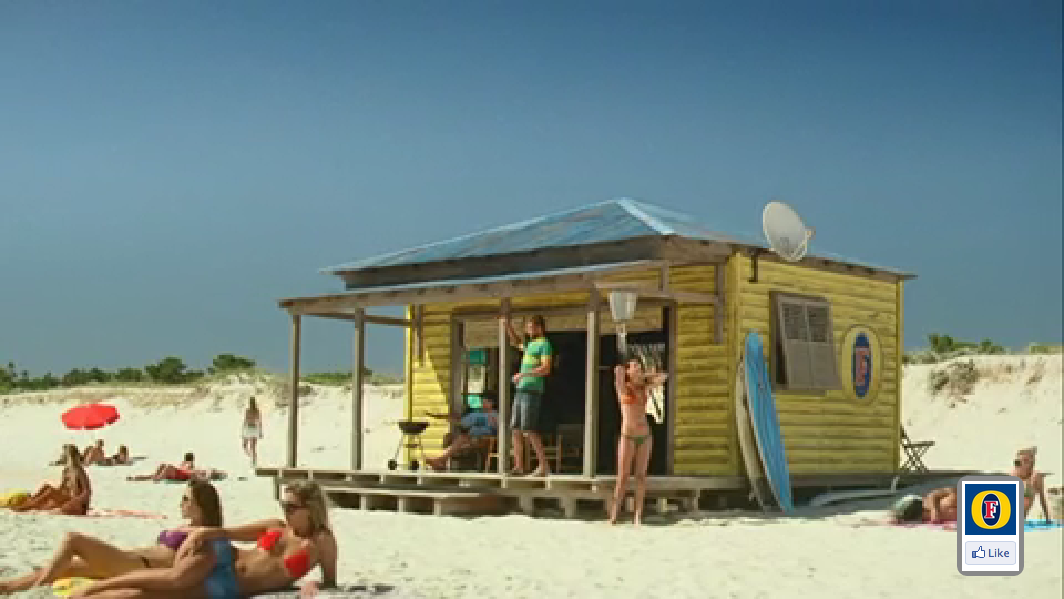
\includegraphics[width=\textwidth,height=0.5\textheight,keepaspectratio]{images/adverts/fosters-1.png}
		\caption{Fosters advert, before liking.}
		\label{fig:fosters1}
	\end{figure}

	\begin{figure}[th]
		\centering
		
\includegraphics[width=\textwidth,height=0.5\textheight,keepaspectratio]{images/adverts/fosters-2.png}
		\caption{Fosters advert, after liking.}
		\label{fig:fosters2}
	\end{figure}

	\subsubsection*{A sample of responses to the interactive advert}
	\begin{enumerate}
		\item{``It was nice to be able to like it there and then.''}
		\item{``Good way to remember to look it up later.''}
		\item{``I found that I was paying more attention because I was hunting for interaction.''}
		\item{``I didn't like it because I don't drink Fosters.''}
	\end{enumerate}

\clearpage
\subsection{Dominoes}
	\begin{description}
		\item[On Load]{Modified Dominoes logo shown in top left including the phrase ``Fancy Domino's Pizza? Tap here!'' See Figure~\ref{fig:Dominos1}.}
		\item[On Tapping the logo]{Logo is replaced by a Pizza cut into 4 sections, each annotated with the phrase ``Tap to Order''. Each section displays a different type of dominoes Pizza. See Figure~\ref{fig:Dominos2}.}
		\item[On Tapping a Pizza Segment]{The graphic is removed and text is displayed reading: ``Your Pizza is on its way!'' See Figure~\ref{fig:Dominos3}.}
		\item[On Timeout]{Text fades away leaving the advert unobstructed.}
	\end{description}

	\begin{figure}[th]
		\centering
		
\includegraphics[width=\textwidth,height=0.5\textheight,keepaspectratio]{images/adverts/dominos-1.png}
		\caption{Domino's advert, before interaction.}
		\label{fig:Dominos1}
	\end{figure}

	\begin{figure}[th]
		\centering
		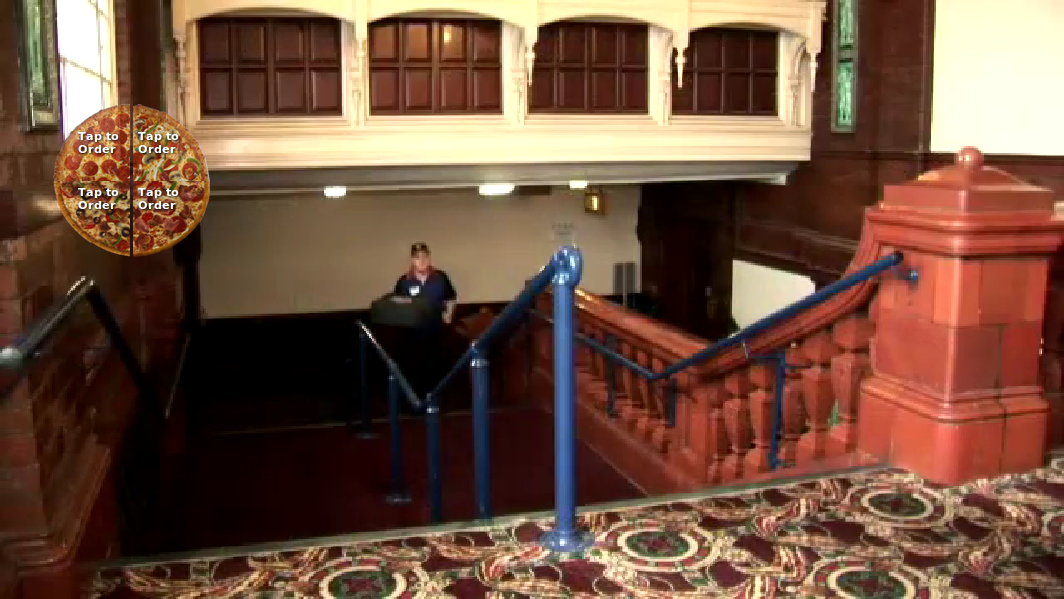
\includegraphics[width=\textwidth,height=0.5\textheight,keepaspectratio]{images/adverts/dominos-2.png}
		\caption{Domino's advert, after the logo is tapped.}
		\label{fig:Dominos2}
	\end{figure}

	\begin{figure}[th]
		\centering
		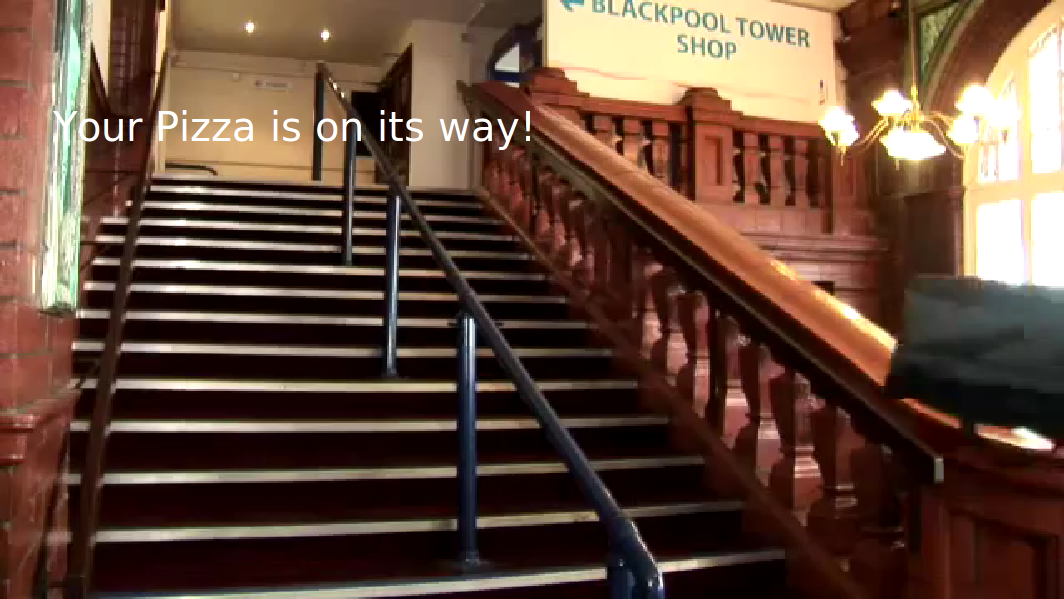
\includegraphics[width=\textwidth,height=0.5\textheight,keepaspectratio]{images/adverts/dominos-3.png}
		\caption{Domino's advert, after selecting a pizza segment.}
		\label{fig:Dominos3}
	\end{figure}
	
	\subsubsection*{A sample of responses to the interactive advert}
	\begin{enumerate}
		\item{``Interaction did not last long enough, so I got bored.''}
		\item{``I love the idea of being able to order a Pizza right from the advert. I was a little disappointed the whole menu was not there.''}
		\item{``There should at least be a confirm button, being able to order a Pizza in two clicks is a bit scary.''}
		\item{One participant who attended on Tuesday mumbled ``Ah it's two for Tuesdays as well.''}
		\item{``Having already seen it in the first session, the interaction gave me something to do, it's only a shame it was so short.''}
		\item{I interacted in the vain hope that it would go away, it went on forever.''}
		\item{``The interaction made me pay a bit more attention. Now I really want a Domino's.''}
	\end{enumerate}

\clearpage
\subsection{Unified Insurance Cover}
	\begin{description}
		\item[On Load]{Grey, semi-transparent bar displayed along the bottom of the screen with the text ``I have...'' positioned at the left. Additionally another similar box appears in the top right with the text ``Your Quote: £0''. See Figure~\ref{fig:Paddy1}.}
		\item[On Timeout Event]{A tickbox appears first growing then shrinking into place to the right of the current content in the lower bar marked ``A laptop?'' See Figure~\ref{fig:Paddy2}.}
		\item[On Timeout Event]{A tickbox appears first growing then shrinking into place to the right of the current content in the lower bar marked ``A hifi?'' See Figure~\ref{fig:Paddy3}.}
		\item[On Timeout Event]{A tickbox appears first growing then shrinking into place to the right of the current content in the lower bar marked ``A bike?'' See Figure~\ref{fig:Paddy4}.}
		\item[On Timeout Event]{A tickbox appears first growing then shrinking into place to the right of the current content in the lower bar marked ``A console?'' See Figure~\ref{fig:Paddy5}.}
		\item[On ticking or unticking a tickbox]{The quote in the top right changes to reflect an estimated quote for someone with the items currently ticked. See Figure~\ref{fig:Paddy6} and Figure~\ref{fig:Paddy7}.}
	\end{description}

	\begin{figure}[th]
		\centering
		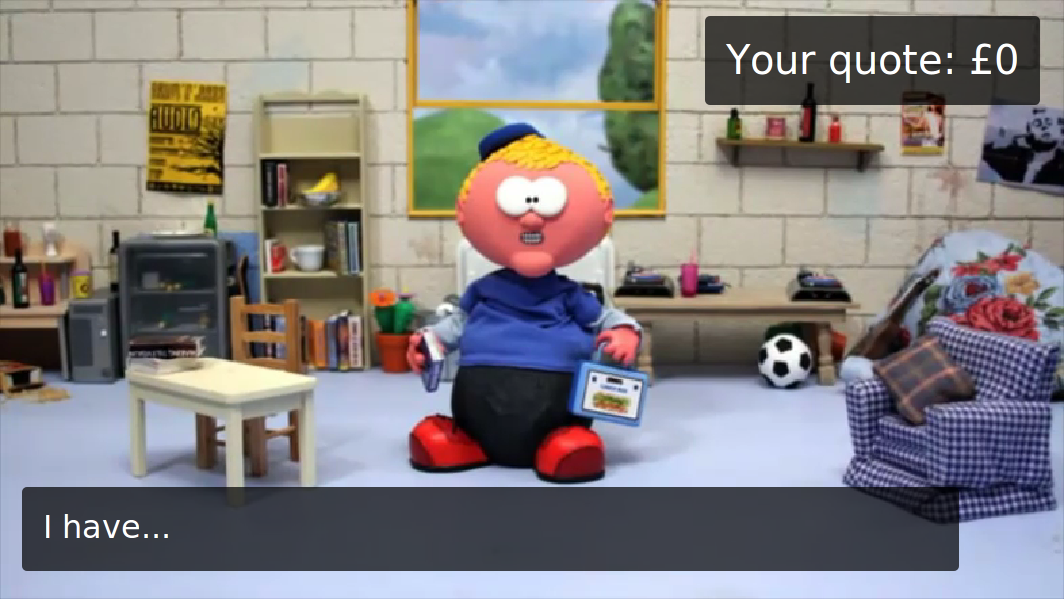
\includegraphics[width=\textwidth,height=0.5\textheight,keepaspectratio]{images/adverts/unified_insurance_cover-1.png}
		\caption{Unified Insurance Cover advert, initial.}
		\label{fig:Paddy1}
	\end{figure}

	\begin{figure}[th]
		\centering
		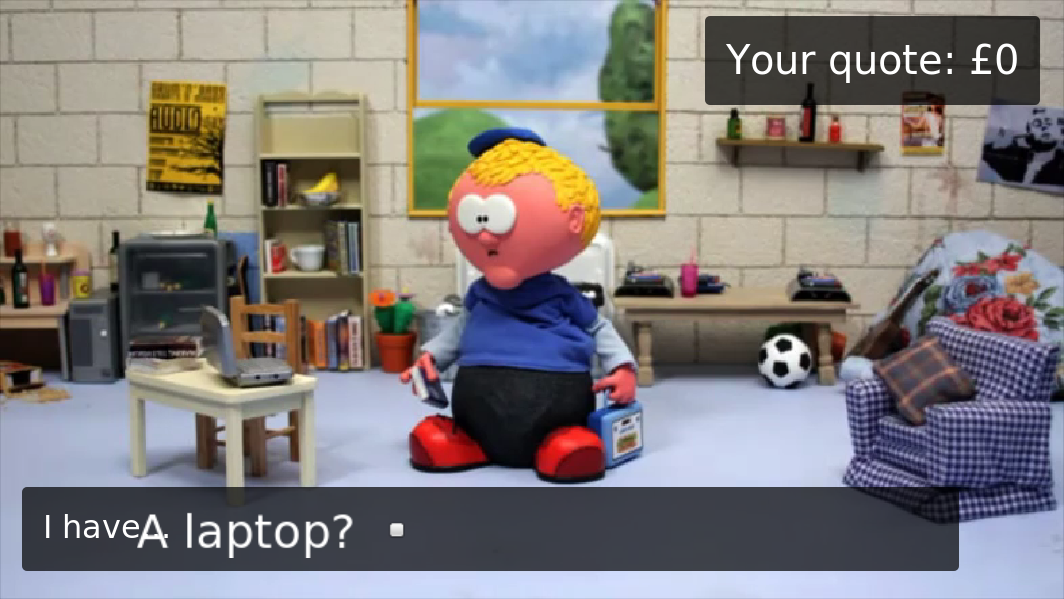
\includegraphics[width=\textwidth,height=0.5\textheight,keepaspectratio]{images/adverts/unified_insurance_cover-2.png}
		\caption{Unified Insurance Cover advert, first item added.}
		\label{fig:Paddy2}
	\end{figure}

	\begin{figure}[th]
		\centering
		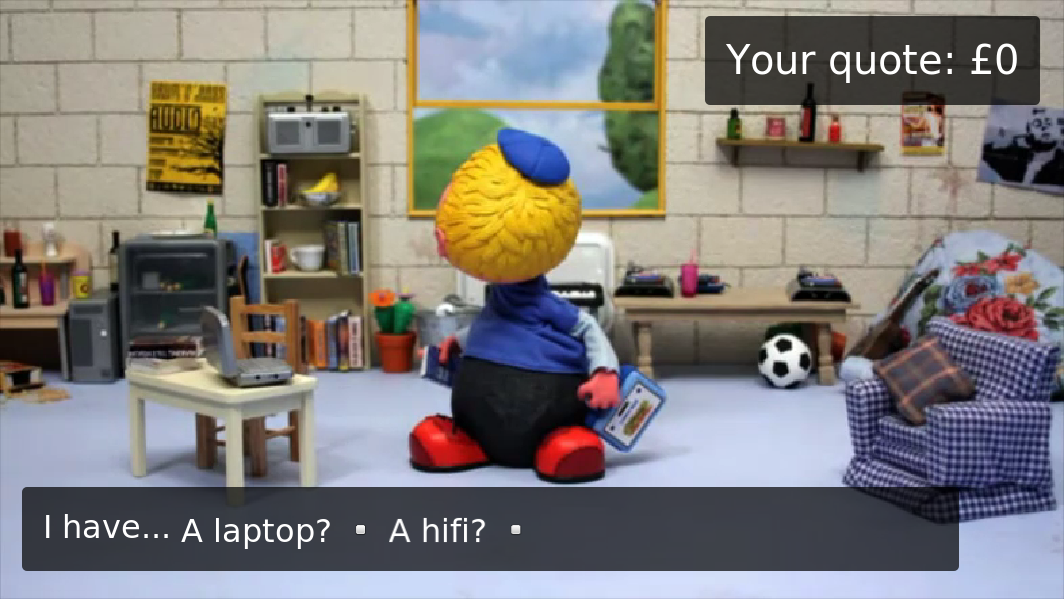
\includegraphics[width=\textwidth,height=0.5\textheight,keepaspectratio]{images/adverts/unified_insurance_cover-3.png}
		\caption{Unified Insurance Cover advert, second item added.}
		\label{fig:Paddy3}
	\end{figure}

	\begin{figure}[th]
		\centering
		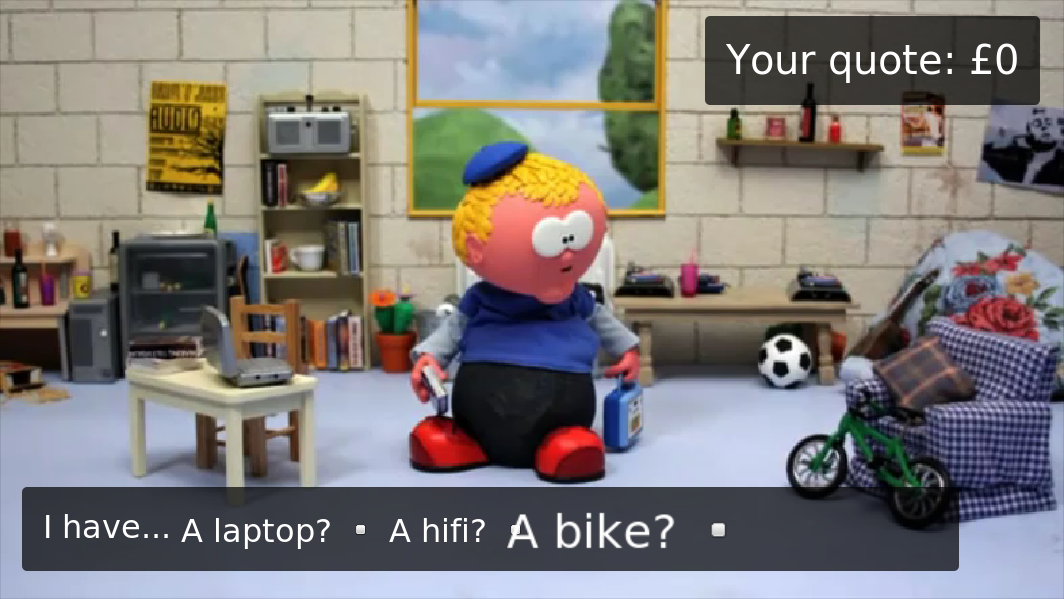
\includegraphics[width=\textwidth,height=0.5\textheight,keepaspectratio]{images/adverts/unified_insurance_cover-4.png}
		\caption{Unified Insurance Cover advert, third item added.}
		\label{fig:Paddy4}
	\end{figure}

	\begin{figure}[th]
		\centering
		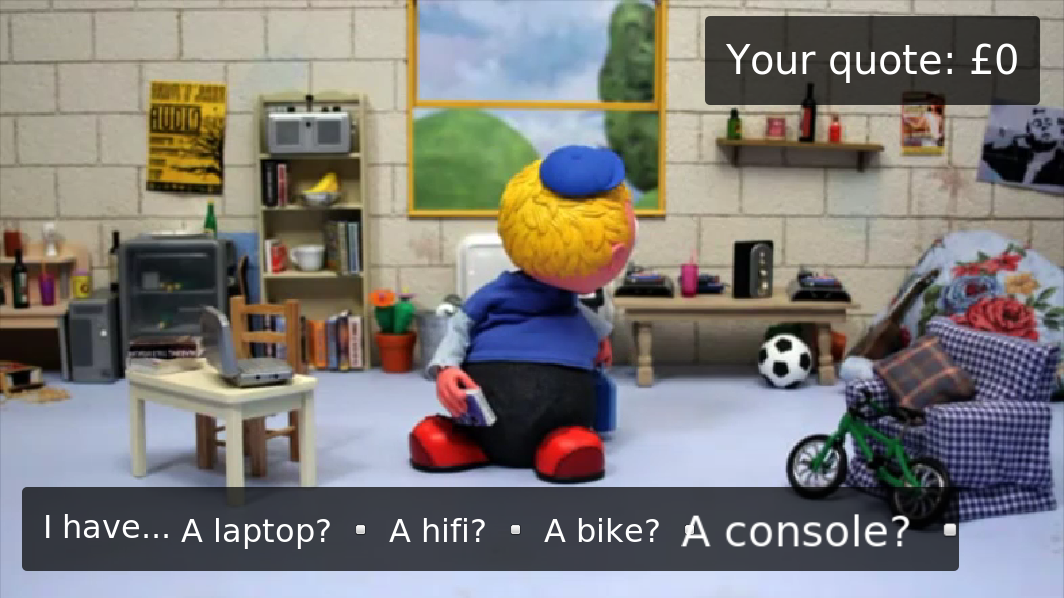
\includegraphics[width=\textwidth,height=0.5\textheight,keepaspectratio]{images/adverts/unified_insurance_cover-5.png}
		\caption{Unified Insurance Cover advert, fourth item added.}
		\label{fig:Paddy5}
	\end{figure}

	\begin{figure}[th]
		\centering
		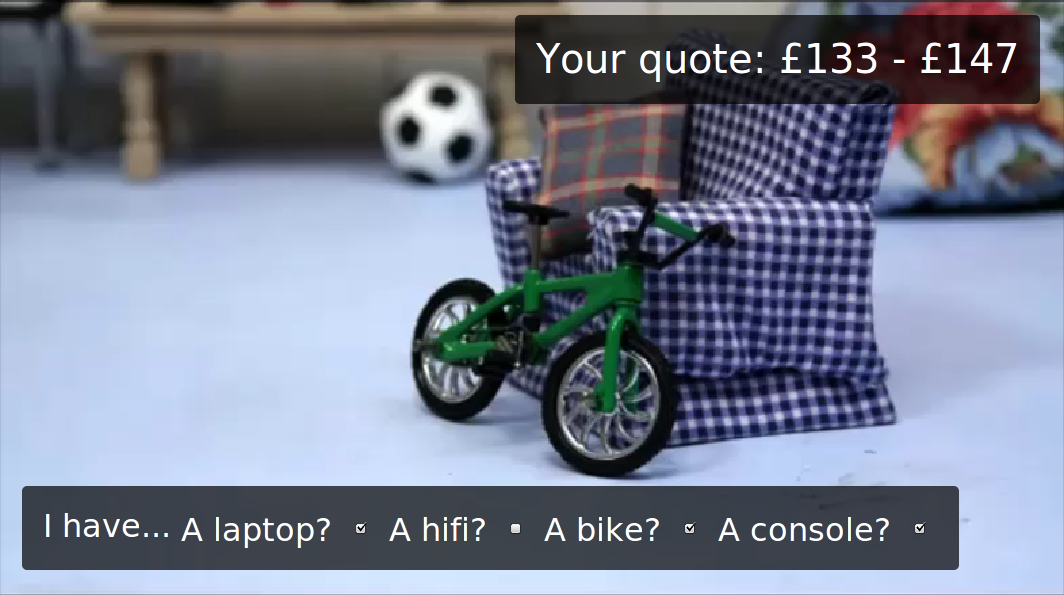
\includegraphics[width=\textwidth,height=0.5\textheight,keepaspectratio]{images/adverts/unified_insurance_cover-6.png}
		\caption{Unified Insurance Cover advert, several items ticked.}
		\label{fig:Paddy6}
	\end{figure}

	\begin{figure}[th]
		\centering
		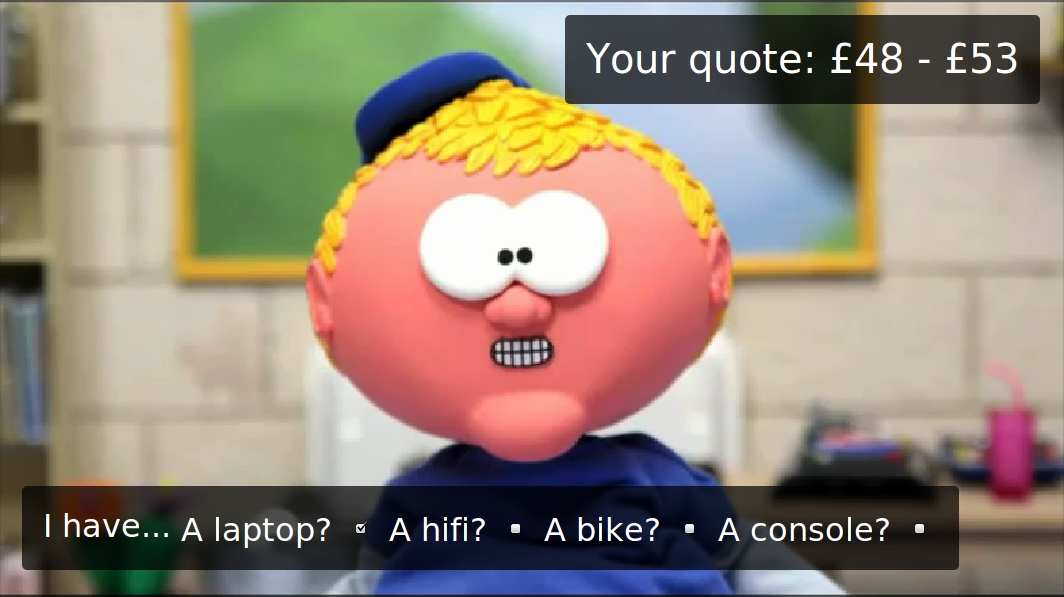
\includegraphics[width=\textwidth,height=0.5\textheight,keepaspectratio]{images/adverts/unified_insurance_cover-7.png}
		\caption{Unified Insurance Cover advert, single item ticked.}
		\label{fig:Paddy7}
	\end{figure}
	
	\subsubsection*{A sample of responses to the interactive advert}
	\begin{enumerate}
		\item{``It was interesting to see the sort of quote I would get, especially since I am thinking of changing my insurance company next year.''}
		\item{``I interacted with it because I was curious.''}
		\item{``I already saw this advert on TV, the sample quote thing really helped keep my attention on the advert.''}
		\item{``This advert would be amazing if you added a splat the spider game.''}
	\end{enumerate}

\clearpage
\subsection{thetrainline.com}
	\begin{description}
		\item[On Load]{Translucent grey box displayed on the right of the screen with the text ``Are train tickets too expensive?'' and two buttons; one green, marked ``YES'' and one red marked ``NO''. See Figure~\ref{fig:trainline1}}
		\item[On clicking either button]{The buttons are removed and replaced by a bar chart showing live results of the poll. See Figure~\ref{fig:trainline2}}
	\end{description}

	\begin{figure}[th]
		\centering
		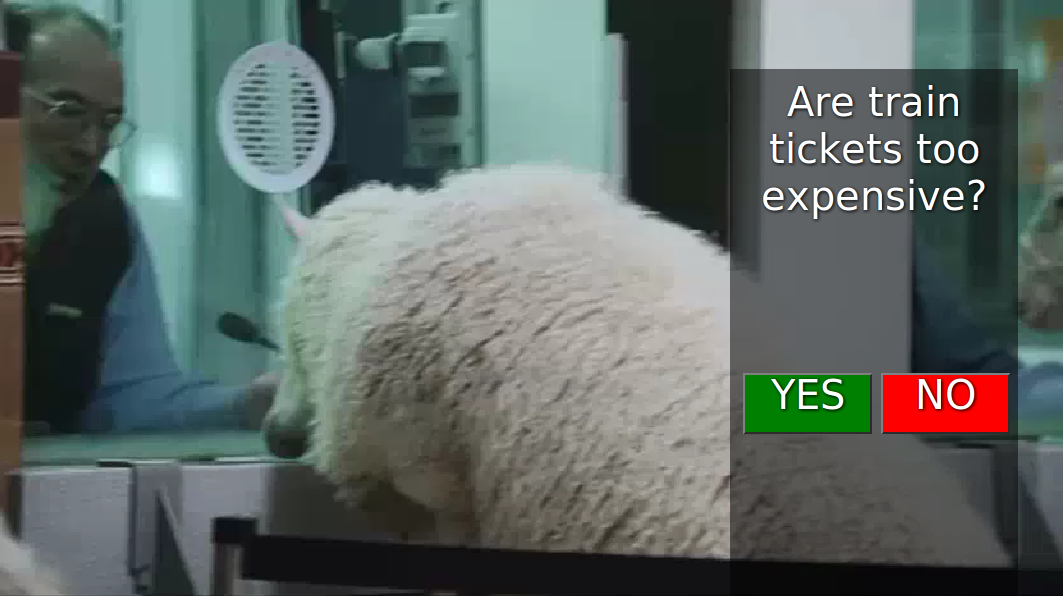
\includegraphics[width=\textwidth,height=0.5\textheight,keepaspectratio]{images/adverts/trainline-1.png}
		\caption{thetrainline.com advert, before interaction.}
		\label{fig:trainline1}
	\end{figure}

	\begin{figure}[th]
		\centering
		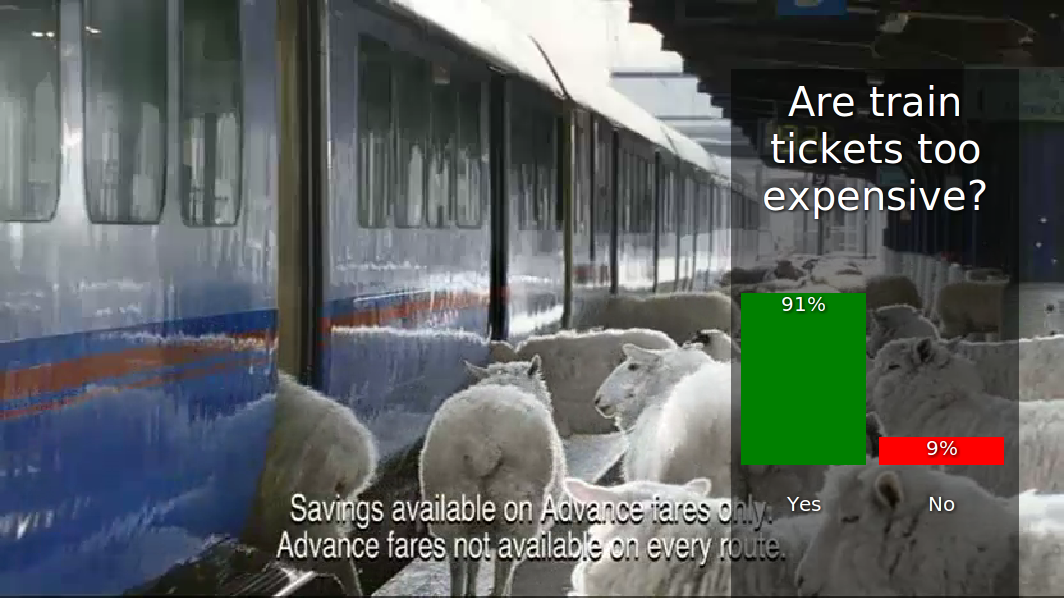
\includegraphics[width=\textwidth,height=0.5\textheight,keepaspectratio]{images/adverts/trainline-2.png}
		\caption{thetrainline.com advert, after option is selected.}
		\label{fig:trainline2}
	\end{figure}
	
	\subsubsection*{A sample of responses to the interactive advert}
	\begin{enumerate}
		\item{``I interacted because, well it's true!''}
		\item{``I thought it was cool seeing the results of the poll in the advert.''}
		\item{``I was shocked that anyone answered no to that!''}
		\item{``I wish I could have hidden the interactive stuff after I was done with it.''}
	\end{enumerate}

\clearpage
\subsection{Pot Noodle}
	\begin{description}
		\item[On Load]{Grey, semi-transparent bar displayed along the bottom of the screen with the text ``BEST Pot Noodle?''. Images of 5 flavours of Pot Noodle are displayed next to this as well as a 6th image in the shape of a Pot Noodle with a ``?'' in the centre. A countdown also begins starting at ``15s'' positioned below the text. See Figure~\ref{fig:potNoodle1}.}
		\item[Every second for 15 seconds]{Countdown text updates to show 1 less second remaining.}
		\item[If user clicks a Pot Noodle image before the countdown ends]{The Pot Noodle they selected grows to emphasise that it has been selected. See Figure~\ref{fig:potNoodle2}.}
		\item[If user clicks the same Pot Noodle image before the countdown ends that they previously selected]{The Pot Noodle they tapped shrinks to its initial size to emphasise that it has been deselected.}
		\item[If user clicks a different Pot Noodle image before the countdown ends than one that they previously selected]{The Pot Noodle they selected before shrinks to its initial size to emphasise that it has been deselected. The new Pot Noodle they selected grows to emphasise that it has been selected. See Figure~\ref{fig:potNoodle3}.}
		\item[If the countdown ends while no Pot Noodle has been chosen]{The grey bar fades out leaving the remainder of the advert unobstructed.}
		\item[If the countdown ends while a pot noodle is selected]{The gray bar fades out and the user is briefly shown some text ``Thanks for voting''. See Figure~\ref{fig:potNoodle4}.}
		\item[On Timeout]{Text fades away leaving the advert unobstructed.}
	\end{description}

	\begin{figure}[th]
		\centering
		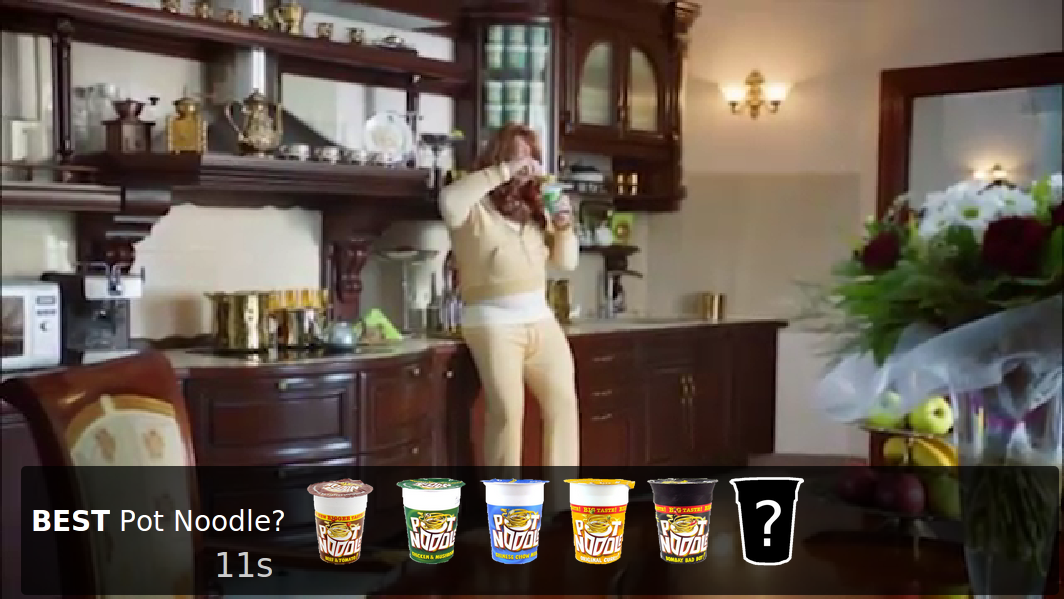
\includegraphics[width=\textwidth,height=0.5\textheight,keepaspectratio]{images/adverts/pot_noodle-1.png}
		\caption{Pot Noodle advert, before interaction.}
		\label{fig:potNoodle1}
	\end{figure}

	\begin{figure}[th]
		\centering
		
\includegraphics[width=\textwidth,height=0.5\textheight,keepaspectratio]{images/adverts/pot_noodle-2.png}
		\caption{Pot Noodle advert, other Pot Noodle selected.}
		\label{fig:potNoodle2}
	\end{figure}

	\begin{figure}[th]
		\centering
		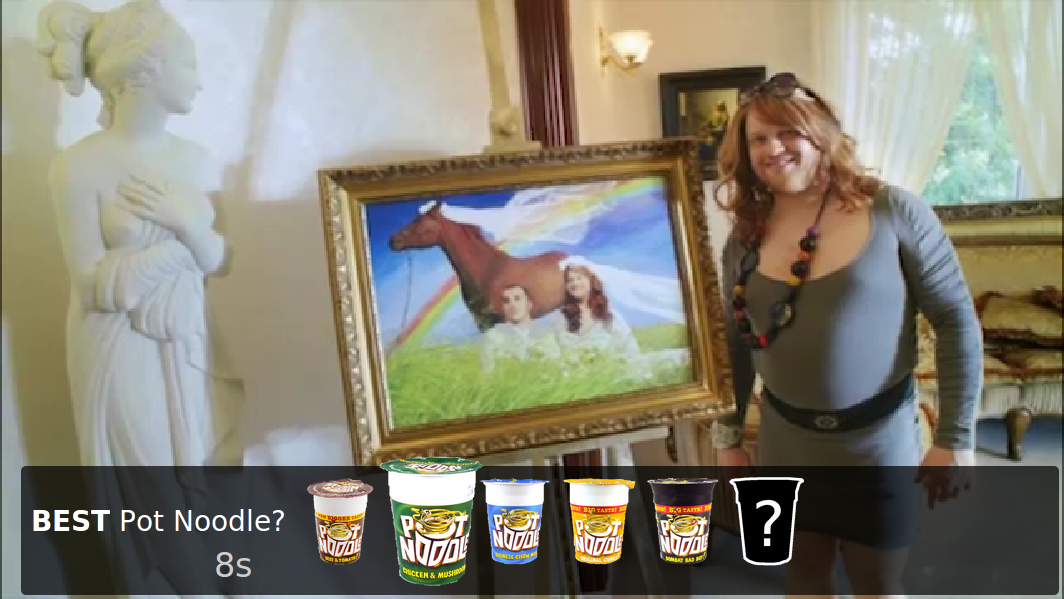
\includegraphics[width=\textwidth,height=0.5\textheight,keepaspectratio]{images/adverts/pot_noodle-3.png}
		\caption{Pot Noodle advert, Chicken and Mushroom Pot Noodle selected.}
		\label{fig:potNoodle3}
	\end{figure}

	\begin{figure}[th]
		\centering
		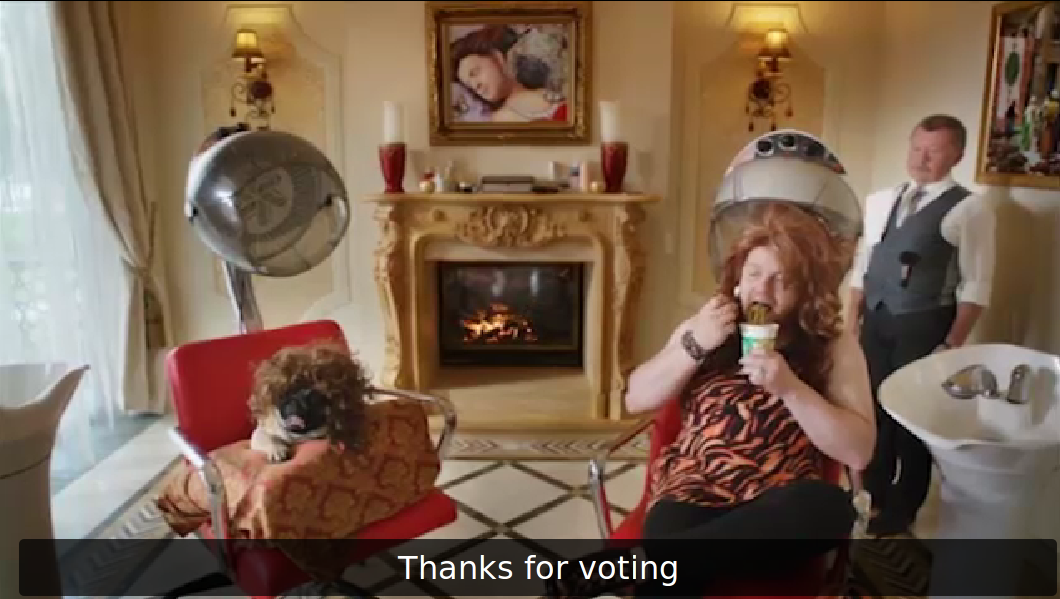
\includegraphics[width=\textwidth,height=0.5\textheight,keepaspectratio]{images/adverts/pot_noodle-4.png}
		\caption{Pot Noodle advert, after countdown ends.}
		\label{fig:potNoodle4}
	\end{figure}
	
\subsubsection*{A sample of responses to the interactive advert}
	\begin{enumerate}
		\item{``I wish it had shown me the results of the poll like the trainline one did.''}
		\item{``I felt pressured by the timer on screen.''}
		\item{``I found the advert horrifying! At least the little favourite Pot Noodle thing gave me something else to do. I don't think I will ever forget that spray tan.''}
		\item{``I don't like Pot Noodle so I did not want to vote.''}
	\end{enumerate}

\clearpage
\subsection{Smirnoff}
	\begin{description}
		\item[On Load]{A Facebook ``Like'' button is present in the lower right hand part of the screen. See Figure~\ref{fig:smirnoff1}.}
		\item[On Clicking the ``Like Button'']{``Like'' button visually changes to indicate that the product has been liked. See Figure~\ref{fig:smirnoff2}.}
	\end{description}

	\begin{figure}[th]
		\centering
		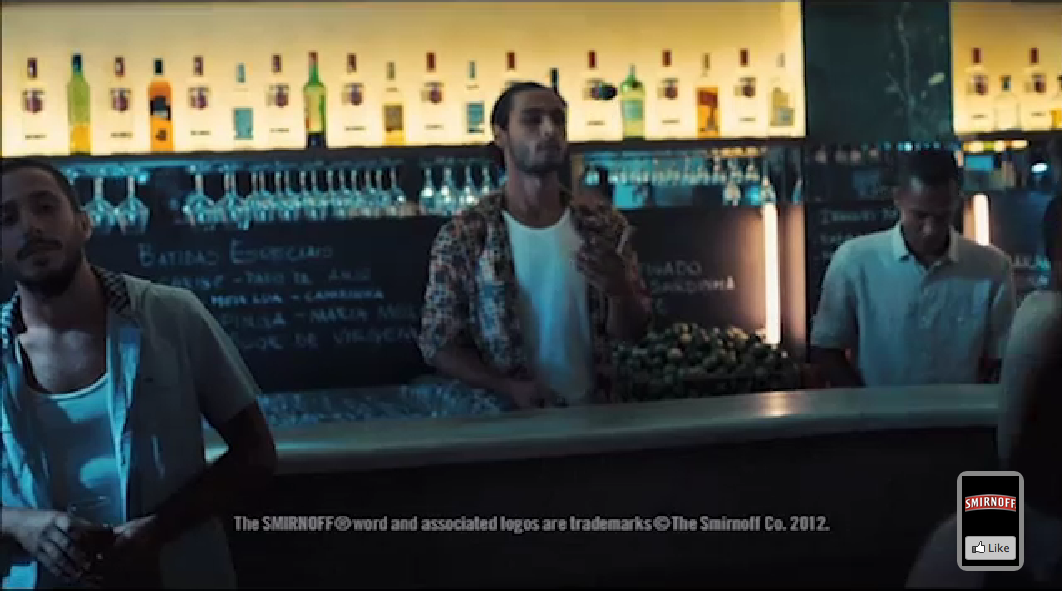
\includegraphics[width=\textwidth,height=0.5\textheight,keepaspectratio]{images/adverts/smirnoff-1.png}
		\caption{Smirnoff advert, before liking.}
		\label{fig:smirnoff1}
	\end{figure}

	\begin{figure}[th]
		\centering
		
\includegraphics[width=\textwidth,height=0.5\textheight,keepaspectratio]{images/adverts/smirnoff-2.png}
		\caption{Smirnoff advert, after liking.}
		\label{fig:smirnoff2}
	\end{figure}
	
	\subsubsection*{A sample of responses to the interactive advert}
	\begin{enumerate}
		\item{``I wish there were less alcohol adverts. I don't drink.''}
		\item{``I don't drink Smirnoff.''}
		\item{``The button was a bit hard to see, I only noticed it right at the end.''}
		\item{``I liked the little like buttons.''}
	\end{enumerate}

\clearpage
\subsection{The Perks of Being a Wallflower}
	\begin{description}
		\item[On Load]{Grey, semi-transparent box displayed in the bottom left of the screen with the text ``Find nearby showings:''. Below this is a box with helper text ``postcode'' and to the right of this is a button marked ``Go''. See Figure~\ref{fig:wallflower1}.}
		\item[On clicking the ``Go'' button with a valid postcode in the postcode box]{A map is displayed, centred on the screen with markers indicating nearby cinemas showing the film. The map window comes with its own set of standard controls which may also be used. See Figure~\ref{fig:wallflower2} and Figure~\ref{fig:wallflower3}.}
		\item[On clicking the markers on the map]{A bubble appears over the marker stating the name of the cinema. See Figure~\ref{fig:wallflower4}.}
		\item[On clicking the ``X'' button]{The map view is closed, allowing the advert to be fully seen once more.}
	\end{description}

	\begin{figure}[th]
		\centering
		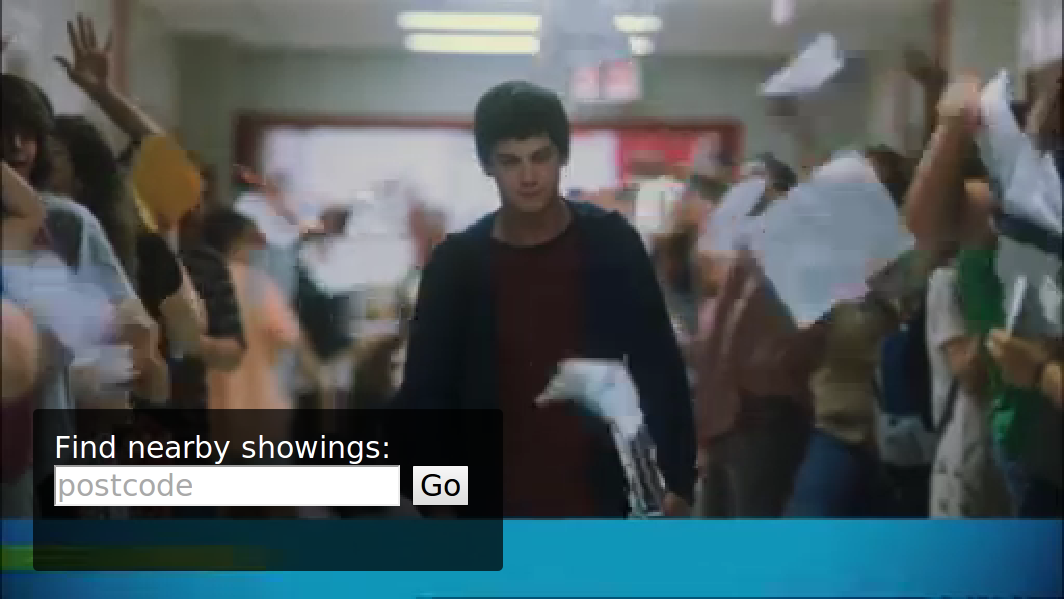
\includegraphics[width=\textwidth,height=0.5\textheight,keepaspectratio]{images/adverts/wallflower-1.png}
		\caption{The Perks of Being a Wallflower film advert, initial.}
		\label{fig:wallflower1}
	\end{figure}

	\begin{figure}[th]
		\centering
		
\includegraphics[width=\textwidth,height=0.5\textheight,keepaspectratio]{images/adverts/wallflower-2.png}
		\caption{The Perks of Being a Wallflower film advert, entered text.}
		\label{fig:wallflower2}
	\end{figure}

	\begin{figure}[th]
		\centering
		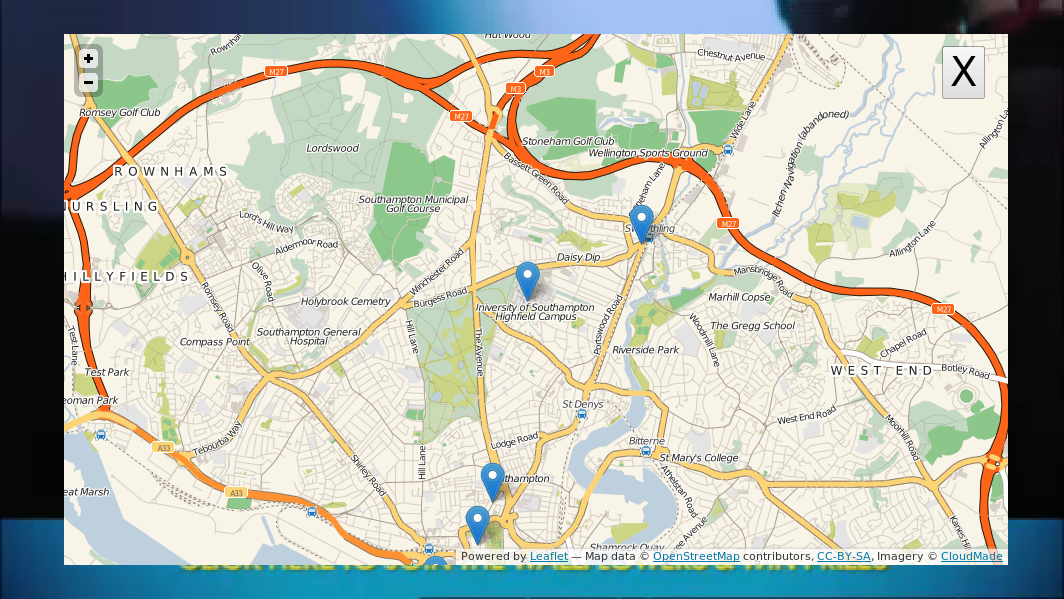
\includegraphics[width=\textwidth,height=0.5\textheight,keepaspectratio]{images/adverts/wallflower-3.png}
		\caption{The Perks of Being a Wallflower film advert, map shown.}
		\label{fig:wallflower3}
	\end{figure}

	\begin{figure}[th]
		\centering
		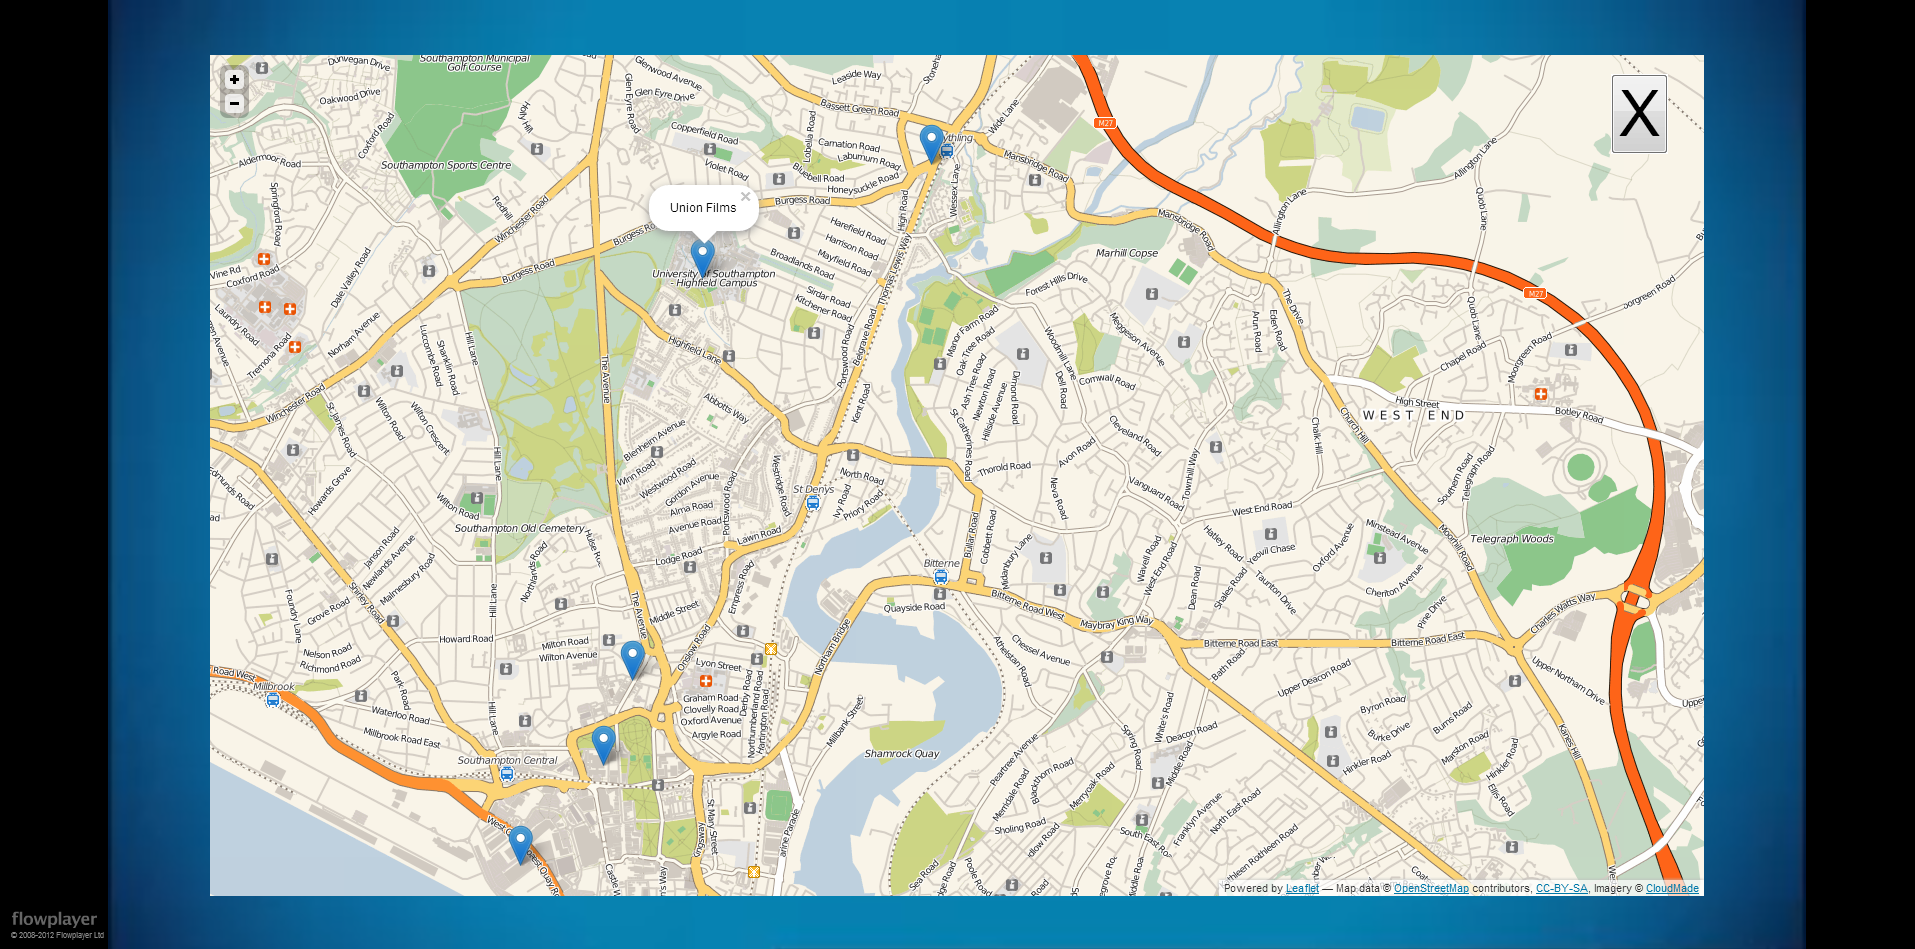
\includegraphics[width=\textwidth,height=0.5\textheight,keepaspectratio]{images/adverts/wallflower-4.png}
		\caption{The Perks of Being a Wallflower film advert, clicked on marker.}
		\label{fig:wallflower4}
	\end{figure}

	\subsubsection*{A sample of responses to the interactive advert}
	\begin{enumerate}
		\item{``I am really not interested in that film, I wish there had been something else to do like on your other adverts.''}
		\item{``That showings finder thing was really useful, I wish it had showing times on it as well though.''}
		\item{``Why wasn't there a like button on this film, I love Emma Watson!''}
		\item{``I was stressed out when I mistyped my postcode that I would not finish in time.''}
		\item{``The advert should pause when you interact so you have more time.''}
		\item{``The interactive stuff took up too much space, couldn't you just have a button to press to give it your post code.''}
	\end{enumerate}

\clearpage
\subsection{Visit Scotland}
	\begin{description}
		\item[On Load]{Grey, semi-transparent bar displayed along the bottom of the screen with the text ``Planning a trip?''. To the right of this is a text box with helper text ``enter your email address'', a button marked ``email me'' and finally a ``X'' button. See Figure~\ref{fig:visit_scotland1}.}
		\item[On clicking the ``X'' button]{The grey box fades out.}
		\item[On clicking ``email me'' with an email address in the email text box]{The controls in the bar are removed and replaced with the text ``Thank you''. See Figure~\ref{fig:visit_scotland2} and Figure~\ref{fig:visit_scotland3}.}
		\item[On Timeout]{Text fades away leaving the advert unobstructed.}
	\end{description}

	\begin{figure}[th]
		\centering
		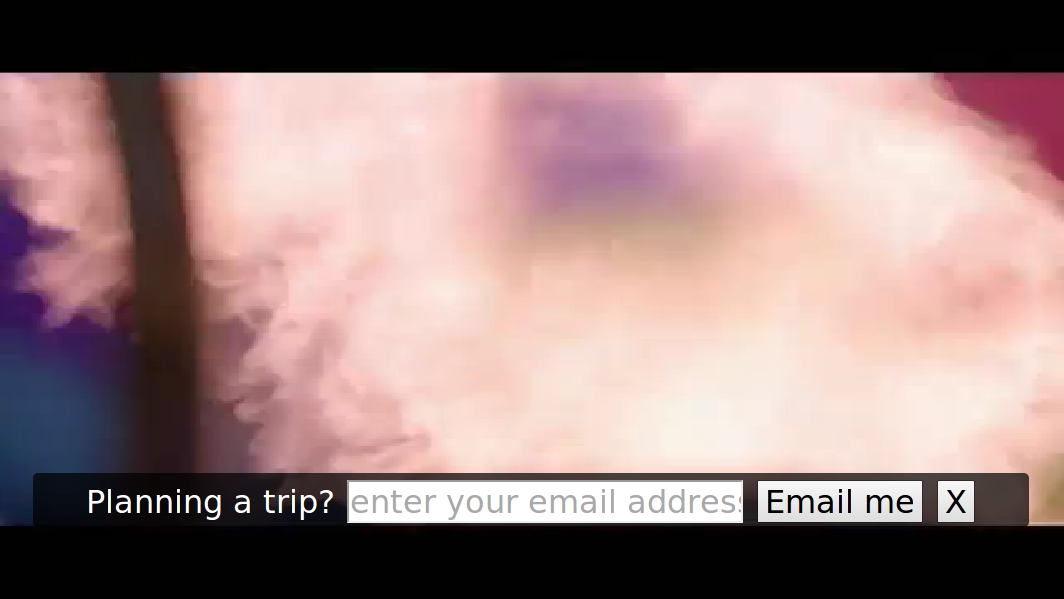
\includegraphics[width=\textwidth,height=0.5\textheight,keepaspectratio]{images/adverts/visit_scotland-1.png}
		\caption{Visit Scotland advert, initial.}
		\label{fig:visit_scotland1}
	\end{figure}

	\begin{figure}[th]
		\centering
		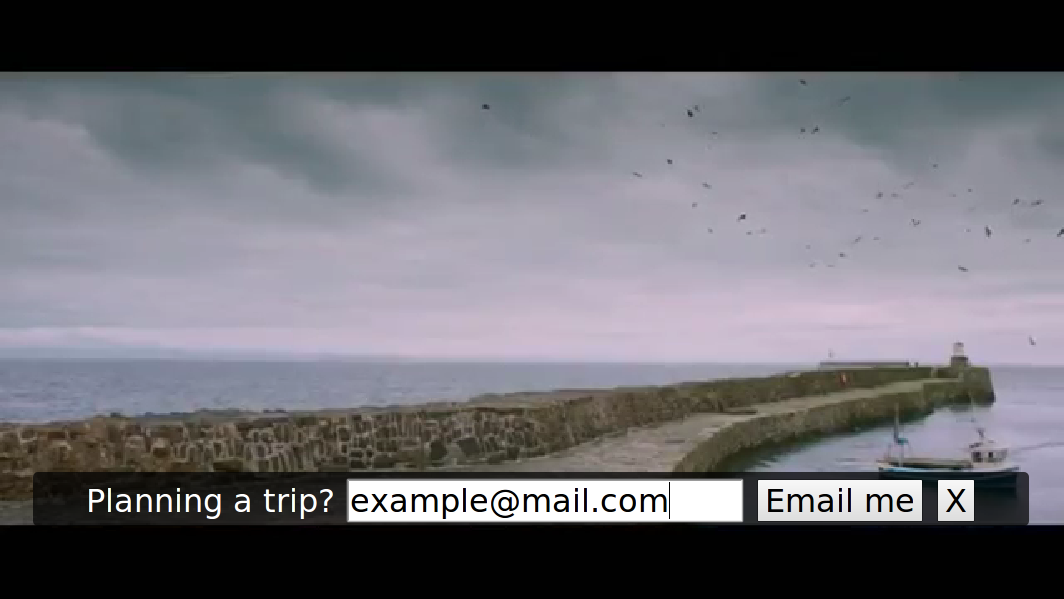
\includegraphics[width=\textwidth,height=0.5\textheight,keepaspectratio]{images/adverts/visit_scotland-2.png}
		\caption{Visit Scotland advert, email entered.}
		\label{fig:visit_scotland2}
	\end{figure}

	\begin{figure}[th]
		\centering
		
\includegraphics[width=\textwidth,height=0.5\textheight,keepaspectratio]{images/adverts/visit_scotland-3.png}
		\caption{Visit Scotland advert, email submitted.}
		\label{fig:visit_scotland3}
	\end{figure}

\subsubsection*{A sample of responses to the interactive advert}
	\begin{enumerate}
		\item{``I did not want to give it my email, I hate being spammed.''}
		\item{``I liked that I could close the interactive bit, I am not planning a holiday any time soon so it was a bit irrelevant.''}
		\item{``I am not planning a holiday but if I was I might have put my email in.''}
		\item{``I felt a bit stressed, my email is really long and I did not know how long I had.''}
	\end{enumerate}
